\documentclass[a4paper,11pt]{article}
\input{/home/tof/Documents/Cozy/latex-include/preambule_doc.tex}
\input{/home/tof/Documents/Cozy/latex-include/preambule_commun.tex}
\newcommand{\showprof}{show them}  % comment this line if you don't want to see todo environment
\setlength{\fboxrule}{0.8pt}
\fancyhead[L]{\fbox{\Large{\textbf{TraitDon 01}}}}
\fancyhead[C]{\textbf{Applications Android}}
\newdate{madate}{10}{09}{2020}
%\fancyhead[R]{\displaydate{madate}} %\today
%\fancyhead[R]{Seconde - SNT}
\fancyhead[R]{Première - NSI}
%\fancyhead[R]{Terminale - NSI}
\fancyfoot[L]{\vspace{1mm}Christophe Viroulaud}
\AtEndDocument{\label{lastpage}}
\fancyfoot[C]{\textbf{Page \thepage/\pageref{lastpage}}}
\fancyfoot[R]{\includegraphics[width=2cm,align=t]{/home/tof/Documents/Cozy/latex-include/cc.png}}

\begin{document}
%DODO problématique: faire un moteur de recherche + revoir la validation des données + remplacer l'exemple notes.csv par un googleplaystore.csv très simplifié (4 lignes, 3 attributs) + ajouter dans le open: encoding="utf8" (et expliquer + ouverture du fichier dans libreoffice avec mauvais encodage <-- occasion de faire utf8???)
%zip sur site: googleplaystore.csv, specifications-app.csv, notes.csv
\section{Problématique}
Devant la multitude d'applications disponibles, il peut être difficile d'effectuer son choix. Des critères (notes, commentaires\dots) permettent cependant de les classer et un moteur de recherche aidera l'utilisateur à faire son choix.
\begin{center}
    \centering
    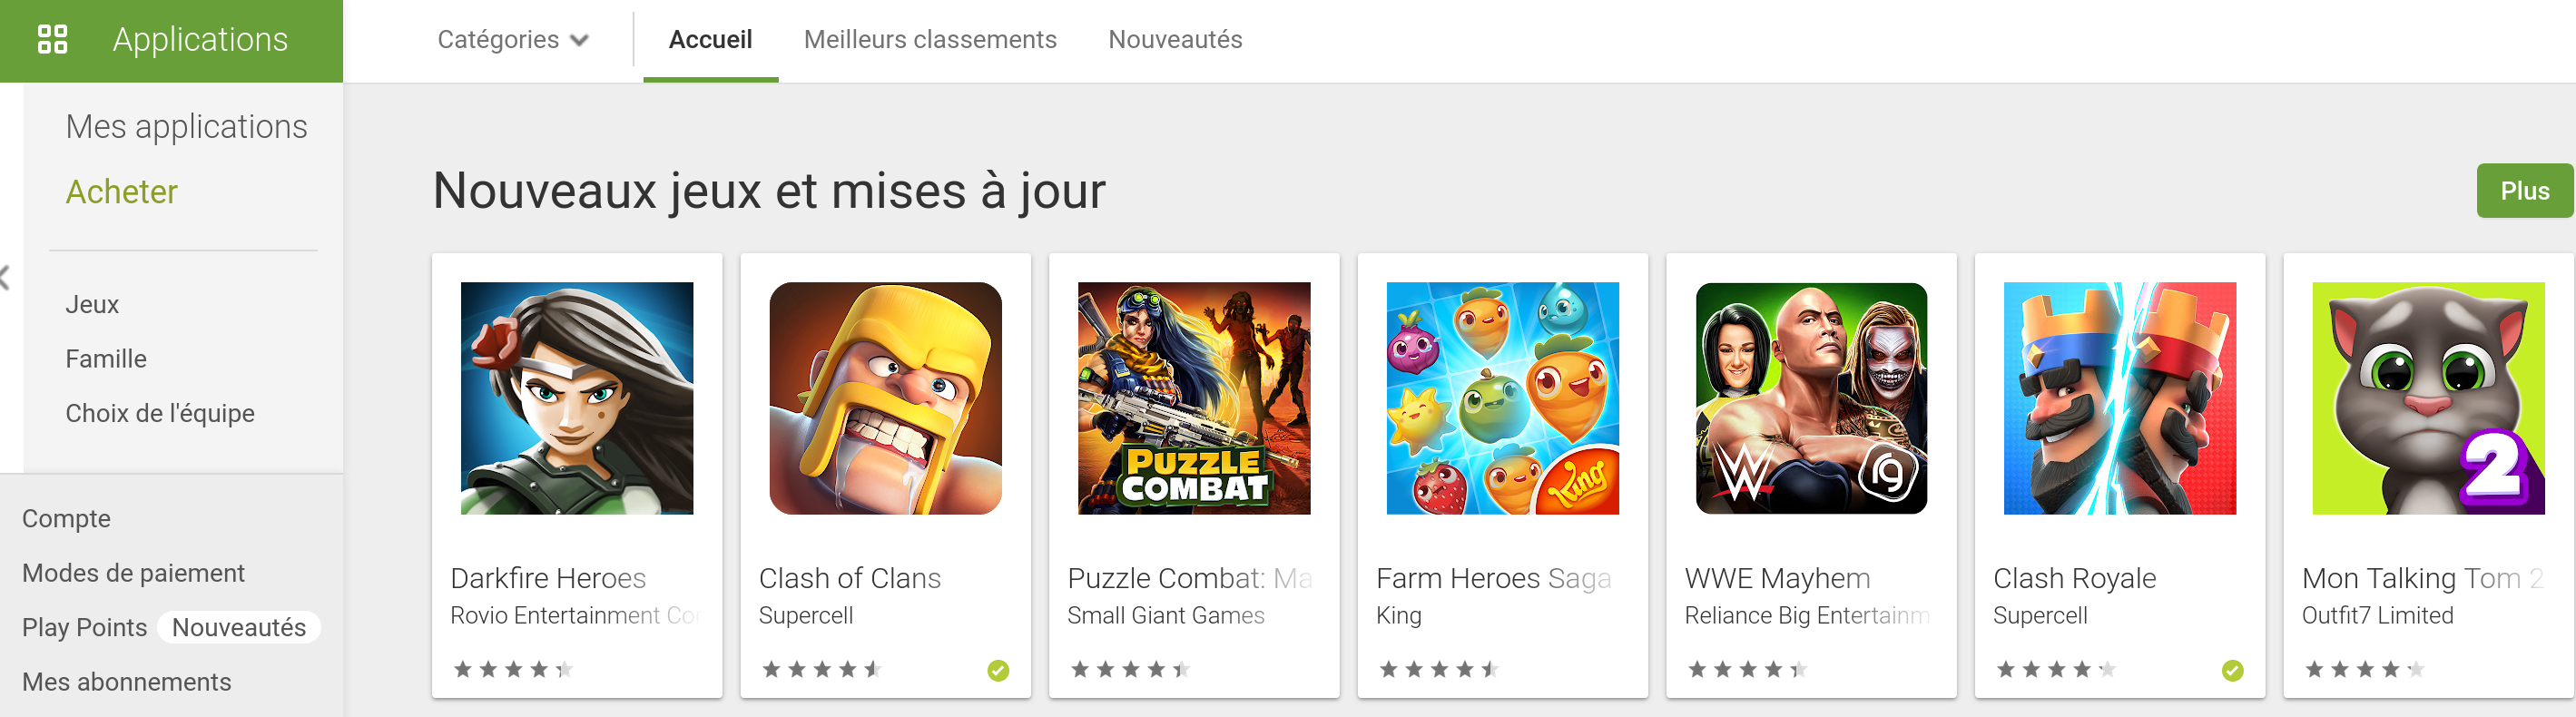
\includegraphics[width=8cm]{ressources/playstore.png}
    \captionof{figure}{Magasin d'applications}
    \label{IMG}
\end{center}
Les informations sont stockées dans un \emph{jeu de données}. Cela peut être un simple fichier texte où chaque ligne contiendra les informations pour une application.
%img aperçu csv
\begin{center}
    \framebox{Comment manipuler un jeu de données?}
\end{center}
%dataset
\section{Données en table}
\subsection{Présentation}
Il est courant de représenter des données sous forme de \emph{table}.
%terme BDD
\begin{center}
    \begin{tabular}{|*{3}{c|}}
        \hline
        \rowcolor{LightGray} Nom & Prénom & Moyenne \\
        \hline
        Turing                   & Alan   & 19      \\
        \hline
        Von Neuman               & John   & 18      \\
        \hline
        Dijkstra                 & Edsger & 17.5    \\
        \hline
        Church                   & Alonso & 19      \\
        \hline
    \end{tabular}
    \captionof{table}{Moyennes des élèves de NSI}
    \label{notes}
\end{center}
Dans le tableau \ref{notes} la première ligne représente les \textbf{attributs} de la table. Ensuite chaque ligne représente un élément (ici un élève) du jeu de données.\\
Pour stocker ces informations on peut utiliser le format de fichiers \emph{csv}.
\begin{aretenir}[]
    Le format \textbf{csv (Comma Separated Values)} permet de stocker des données tabulaires sous forme de valeurs séparées par des \emph{virgules}. Chaque ligne représente un nouvel élément du jeu de données.
    %des fois point-virgules ou tabulation; 1° ligne pas toujours les attributs <- exemple; guillemets pour "encapsuler" (si il y a des virgules dans le texte par ex) json
\end{aretenir}
\begin{activite}
    \begin{enumerate}
        \item Télécharger et décompresser l'annexe \emph{googleplaystore.zip} sur le site \url{https://cviroulaud.github.io}
        \item Ouvrir le fichier \emph{googleplaystore.csv} avec un tableur (LibreOffice).
        \item Repérer les \emph{attributs}.
              %traduire
    \end{enumerate}
\end{activite}
\subsection{Lire un fichier \emph{csv}}
Pour lire un fichier externe dans un programme Python, il faut d'abord ouvrir ce fichier à l'aide de la commande \textbf{\texttt{open}}. Ensuite la bibliothèque \texttt{csv} propose plusieurs méthodes pour itérer sur les lignes du fichier ouvert.
\begin{center}
    \begin{lstlisting}[language=Python]
import csv
# ouvrir le fichier
fichier = open("notes.csv")

lecteur = csv.reader(fichier)
for ligne in lecteur:
    print(ligne)

# libérer le fichier
fichier.close()
\end{lstlisting}
    \captionof{code}{Méthode pour itérer sur les données}
    \label{iterer}
\end{center}
\begin{activite}
    \begin{enumerate}
        \item Tester le code \ref{iterer} dans un fichier \emph{notes.py}.
        \item Remplacer la méthode \textbf{\texttt{reader}} par \textbf{\texttt{DictReader}}.
        \item Quel itérateur semble le plus adapté?
        \item Créer un programme \emph{appgoogle.py}.
        \item Dans le programme, ouvrir le fichier \emph{googleplaystore.csv}.
        \item Créer un tableau de dictionnaires à partir des données du fichier \emph{csv}.
    \end{enumerate}
\end{activite}
%reader et DictReader sont des itérateurs: on ne peut les parcourir qu'une fois
\begin{aretenir}[Commentaire]
    Une variable de type \emph{OrderedDict} sera vue comme un simple dictionnaire.
    % transformer en dict 
\end{aretenir}
\section{Manipuler les données}
\subsection{Valider les données}
Par défaut les données chargées dans un programme par la bibliothèque \textbf{\texttt{csv}} sont des chaînes de caractère. Cependant, certaines des informations comme la note, sont des nombres.
%booléan possible aussi
\begin{activite}
    \begin{enumerate}
        \item Modifier le programme \emph{notes.py}, pour que la moyenne soit stockée comme un flottant.
        \item  Modifier le programme \emph{appgoogle.py} pour typer correctement les informations récoltées.
    \end{enumerate}

    %ValueError: invalid literal for int() with base 10: 'NaN'
    % mettre 0 qd NaN
\end{activite}
\subsection{Rechercher des données}
Une action courante sur un jeu de données est de sélectionner certaines lignes en fonction d'un critère. On peut assimiler cette action au principe général d'un moteur de recherche.
\subsubsection{Sélectionner}
\begin{activite}
    \begin{enumerate}
        \item Écrire la fonction \textbf{\texttt{trouver\_app(mot\_cle: str, tab: list) $\rightarrow$ list}} qui renvoie la liste des applications du tableau \emph{tab} dont le nom contient \emph{mot\_cle}.\\
              \underline{Indication:} L'instruction \textbf{\texttt{in}} permet de vérifier si une sous-chaîne est présente dans une chaîne de caractère.
              %tous les mots commencent par une majuscule
        \item Chercher toutes les applications dont le nom contient le mot \emph{Photo}.
        \item Compter le nombre d'applications renvoyées.
        \item Écrire la fonction \textbf{\texttt{meilleur\_app\_notee(tab: list) $\rightarrow$ dict}} qui renvoie l'application la mieux notée du tableau \emph{tab}.
        \item Trouver l'application photo la mieux notée.
        \item \underline{Pour les plus avancés:} en s'aidant de la documentation, modifier la fonction \textbf{\texttt{trouver\_app}} pour quelle:
              \begin{itemize}
                  \item ne prenne pas en compte la casse des mots,
                  \item renvoie les applications contenant plusieurs mots-clés; les mots sont passés à la fonction par le paramètre \emph{mot\_cle} séparés par un espace.
              \end{itemize}
    \end{enumerate}
\end{activite}
\subsubsection{Agréger}
La sélection précédente étant très restrictive, il peut être intéressant d'offrir un choix plus large. On peut imaginer proposer à l'utilisateur toutes les applications notées au-dessus de la moyenne.
\begin{activite}
    \begin{enumerate}
        \item Écrire la fonction \textbf{\texttt{moyenne\_note(tab: list)  $\rightarrow$ float}} qui calcule la note moyenne des applications de \emph{tab}. Le résultat sera arrondi à deux chiffres significatifs.
        \item Dans le programme principal, construire \emph{par compréhension }le tableau des applications photo dont la note est strictement supérieure à la moyenne.
    \end{enumerate}
\end{activite}
\subsection{Trier des données}
Le tri est une autre opération fréquemment exécutée sur un jeu de données. On peut imaginer dans notre cas, ordonner les applications photo en fonction de leur note. 
\subsubsection{Tri natif}
En tant que langage de haut-niveau Python offre un outil de tri efficace:
\begin{itemize}
    \item la méthode \textbf{\texttt{sort}} trie \emph{en place} un itérable,
    \begin{center}
    \begin{lstlisting}[language=Python]
ma_liste.sort()
    \end{lstlisting}
    \end{center}
    \item la fonction \textbf{\texttt{sorted}} crée un nouvel itérable trié.
    \begin{center}
    \begin{lstlisting}[language=Python]
nouvelle = sorted(ma_liste)   
    \end{lstlisting}
    \end{center}
\end{itemize}
\subsubsection{Clé de tri}
Dans notre cas les objets triés ne sont pas des simples entiers mais des dictionnaires. Il faut alors préciser la \textbf{clé de tri}.
\lstinputlisting[firstline=21 ,lastline=27]{"scripts/tri-cle.py"}
%remarquer que certains ont même note
\begin{activite}
    \begin{enumerate}
        \item Écrire la fonction \textbf{\texttt{parametres\_tri\_1(app: dict) $\rightarrow$ float}} qui renvoie la note de l'application.
        \item Trier le tableau des applications photo en fonction de leur note.
        \item Afficher les cinq meilleures applications.
    \end{enumerate}
    Pour départager les applications avec la même note, on choisit de définir un second paramètre de tri: le nombre de commentaires.
    \begin{enumerate}[resume]
        \item Écrire la fonction \textbf{\texttt{parametres\_tri\_2(app: dict) $\rightarrow$ tuple}} nouvelle clé de tri.
        \item Appliquer cette nouvelle clé.
        \item \underline{Pour les plus avancés:} Reprendre la fonction \textbf{\texttt{tri\_insertion}} et la modifier pour effectuer le tri de la première question.
    \end{enumerate}
    \end{activite}
\end{document}